\documentclass{acm_proc_article-sp}
\usepackage{amsmath}
\usepackage{mathtools}
\usepackage[hidelinks]{hyperref}
\usepackage{amssymb}
\usepackage{tikz}
\usepackage{caption}
\usepackage{graphicx}
\graphicspath{{.}}
\usepackage{listings}
\usepackage{verbatim}
\usepackage{xcolor}
\renewcommand\thefootnote{\textcolor{black}{\arabic{footnote}}}
\hypersetup{colorlinks,urlcolor=blue,citecolor=black}
\usepackage[paper=a4paper,
            %includefoot, % Uncomment to put page number above margin
            marginparwidth=10mm,      % Length of section titles
            marginparsep=0.5mm,       % Space between titles and text
            margin=10mm,              % 25mm margins
            includemp]{geometry}

\begin{document}
\title{``Moneyball'' in NBA to predict the performance of the players}
\numberofauthors{3}
\author{
%
% 1st. author
\alignauthor 
Kirill Novik\\
       \email{kirill.novik@colorado.edu}
% 2nd. author
\alignauthor
Krishna Chaitanya Sripada\\
       \email{krishna.sripada@colorado.edu}
% 3rd. author
\alignauthor
Yu-Ching Kuo\\
       \email{yuching.kuo@colorado.edu}
}
\maketitle
\section*{Task Overview}
The first goal of this project is to assess the goodness of a team based on whether it reaches the playoff or not. By finding the attributes that represent good teams, we can achieve our primary goal which is evaluating the performance of individual players. To accomplish this task, we need to identify parameters that affect the goodness. The datasets we are working with have 26 parameters to choose from, which after reduction becomes only 9. A decision tree approach is applied to find out the most important attributes form the 9 attributes we choose. When the most important attributes are determined, we merge them into one single factor after applying the min-max normalization to these attributes and use it for describing the goodness of a team.
\keywords{Data Mining, Information Gain, Decision Tree, Min-Max Normalization, Accuracy}
\section*{Decision Tree Approach}
From the 26 attributes, we reduce the attributes to 9 attributes which are FG\%, ORB, DRB, AST, STL, BLK, TOV, PF and PTS/G and rule out the attributes that are either redundant or relevant. Here the decision is made based on if a team can make to playoff or not. Information gain for all the 9 attributes we choose are calculated to determine the importance of each attribute. We split the past 30 seasons of NBA league into 20 seasons as a training dataset and 10 seasons as the testing database which has been shown in Figure 1. Within the training dataset, we calculate the information gain for each attribute from the decision tree we construct in Figure 2 for each season and take the average over the past 20 seasons. The results are shown in Figure 3. As can be seen from Figure 3, the top five most critical attributes that can determine the goodness of a team is FG\%, DRB, TOV, PTS/G, and AST respectively due to their high information gain.\\
\begin{equation}
Attribute_{n} = (Attribute - Min) / (Max - Min)
\end{equation}
\textbf{Merge the attributes into a factor (Attribute n+1):}\\
With the goal of using one single factor to describe a team, we need to merge several most critical attributes. Due to the variety of the scale of different attributes, a min-max normalization approach which is shown in Equation 1 where the subscribed N denotes normalized attribute, is applied to unify the scale of various attributes (scale are in 0 $\sim$ 1 after the normalization) and make the merging applicable. An example of normalization is shown in Figure 4 where we normalize the top five most important attributes in the season 2004-2005.

\begin{figure}[!htb]
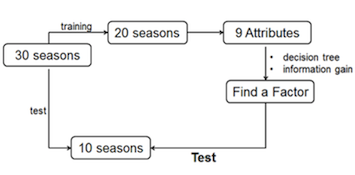
\includegraphics{DatasetTT.png}
\caption{Overview of the analytical model}
\end{figure}

\begin{figure}[!htb]
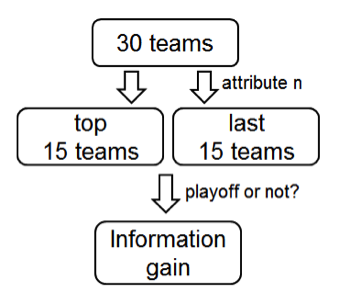
\includegraphics{DT.png}
\caption{Decision Tree Layer-1 for our dataset}
\end{figure}

\begin{figure}[!htb]
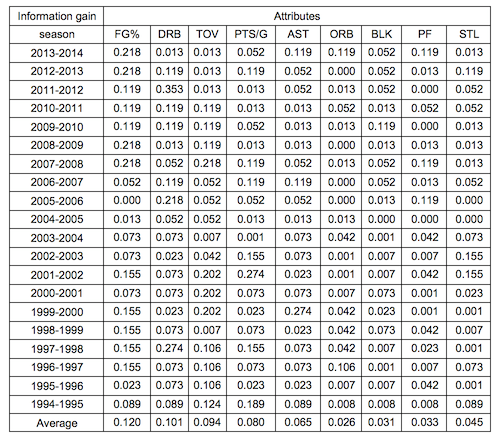
\includegraphics{Table.png}
\caption{The results of information gain in the past 20 seasons}
\end{figure}

\vspace{8em}

\begin{figure}[!htb]
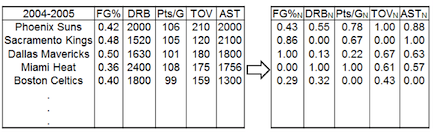
\includegraphics{Norm.png}
\caption{An example of min-max normalization}
\end{figure}

After the normalization, we used Equation 2 to merge the important attributes to generate a mixed factor to describe the goodness of a team which we will name it $Attribute_{n+1}$. When the new attribute ($Attribute_{n+1}$) is found, it will be used to evaluate the NBA teams in each season. For each season, the 30 NBA teams will be split into the top 15 which have the highest value of $Attribute_{n+1}$ and the last 15. In this work, we aim at finding an $Attribute_{n+1}$ that can ensure 80\% of the top 15 teams make to the playoff over the past 30 years.\\
\begin{equation}
Attribute_{n+1} = aFG\%_{n} + bDRB_{n} + cTOV + dPTS/G_{n} + ...
\end{equation}
To find the $Attribute_{n+1}$, the unknown parameters in Equation 2 are required to be found. Since the scale of the normalized attributes are in 0 $\sim$1, we postulate that the unknown parameters are ranging from 0 to 1. For each parameter, a trial and error approach with an interval of 0.01 from 0 to 1 is used for detecting the optimized parameter pair. Here the top two attributes are used for constructing the new factor due to its better accuracy compare to other models which can be found in Figure 5. Within the $10^{4}$ possible combinations of the unknown parameters, the optimized pair is found to be (1.0, 0.6) with the training accuracy to be 79.4\% for 20 seasons (1995-2014) and the prediction accuracy to be 82.0\% for the rest of the 10 seasons.\\
\begin{figure}[!htb]
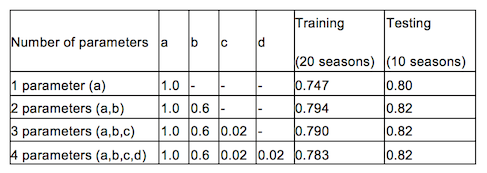
\includegraphics{Accuracy.png}
\caption{The optimized parameters and accuracy for various models}
\end{figure}

\section*{Remaining Work}
\begin{itemize}
\item We will further optimize the $Attribute_{n+1}$ with 5 unknown parameters to check if we can find a better model for finding the new attribute. However, the result from the two-parameter model we have is satisfactory and acceptable for the prediction. 
\item Since several important attributes including FG\%, DRB, TOV, PTS/G, and AST and an optimized factor is found for finding a good team, we will use these attributes to evaluate an individual player. With similar approach and by the evaluation of these attributes and the player's annual income, we may be able to find a new index to describe the goodness of an individual player. We believe that by the new index we are going to find, we will be able to form a cheap but competitive team that is guaranteed to be in the playoff. 
\end{itemize}
\end{document}
